\input{preamble-libroTrabajoGrado0.tex}
% \usepackage{showframe}
%% Title page information for article
\title{Matemáticas Ilustrativas\\
{\large Grado 0 - Unidad 1}}
\author{Adaptación del Grupo LEMA\\
\href{https://www.grupolema.org}{\nolinkurl{https://www.grupolema.org}}
}
\date{March 31, 2025}
\begin{document}
%% bottom alignment is explicit, since it normally depends on oneside, twoside
\raggedbottom
%% Target for xref to top-level element is document start
\label{gra0-uni1}\hypertarget{gra0-uni1}{}
\maketitle
\thispagestyle{empty}
\renewcommand*{\abstractname}{}
\begin{abstract}
Este documento (HTML, pdf, latex o epub) se generó con \href{https://pretextbook.org}{PreTeXt}\footnote{\nolinkurl{pretextbook.org}\label{meta-source-2-2}}. El código fuente con el contenido para generarlo se encuentra en \href{https://github.com/enriqueacosta/IllustrativeMath-GrupoLEMA}{\nolinkurl{github.com/enriqueacosta}}.%
\end{abstract}
\clearpage
\renewcommand*{\abstractname}{Licencia}
\begin{abstract}
2024~Versión PreTeXt, traducciones completas de las guías y adaptaciones © Enrique Acosta (\href{https://enriqueacosta.github.io}{\nolinkurl{enriqueacosta.github.io}}). Iniciativa del Grupo LEMA (\href{https://www.grupolema.org}{\nolinkurl{www.grupolema.org}})Publicado bajo una licencia Creative Commons Attribution-NonCommercial-ShareAlike 4.0 International (CC BY SA NC 4.0).%
\par
En breve e incompleto (los detalles están en las licencias), \alert{tiene toda libertad para adaptar, copiar y distribuir este material siempre y cuando le mantenga la misma licencia, incluya la atribución correspondiente (mencione a Enrique Acosta, al Grupo LEMA, a Illustrative Mathematics y a OpenUp Resources en la forma que se describe a continuación) y lo use para fines no comerciales}.%
\par
Ver detalles de la licencia en \href{https://creativecommons.org/licenses/by-nc-sa/4.0/}{creativecommons.org}\footnote{\nolinkurl{creativecommons.org/licenses/by-nc-sa/4.0/}\label{meta-copyright-6-2}}.%
\par
Además, se permite la impresión y distribución a costo para uso educativo o personal. La reventa comercial o actividades con fines de lucro no están permitidas sin autorización previa.%
\par
Grados K-5 adaptados de IM K–5 Math v.I, ©~2021 Illustrative Mathematics~® \href{https://curriculum.illustrativemathematics.org}{illustrativemathematics.org}\footnote{\nolinkurl{curriculum.illustrativemathematics.org}\label{meta-copyright-8-4}} en su versión en español en \href{https://im.kendallhunt.com/K5_ES/curriculum.html}{im.kendallhunt.com}\footnote{\nolinkurl{im.kendallhunt.com/K5_ES/curriculum.html}\label{meta-copyright-8-6}}, distribuido con una licencia Creative Commons Attribution 4.0 International License (CC BY 4.0). Ver detalles de esta licencia en \href{https://creativecommons.org/licenses/by/4.0/}{creativecommons.org}\footnote{\nolinkurl{creativecommons.org/licenses/by/4.0/}\label{meta-copyright-8-8}}.%
\par
Grados 6-8 adaptados de IM 6–8 v3.1415, ©~2019 Illustrative Mathematics~® \href{https://curriculum.illustrativemathematics.org}{illustrativemathematics.org}\footnote{\nolinkurl{curriculum.illustrativemathematics.org}\label{meta-copyright-9-4}} en su versión en español en \href{https://im.kendallhunt.com/K5_ES/curriculum.html}{im.kendallhunt.com}\footnote{\nolinkurl{im.kendallhunt.com/K5_ES/curriculum.html}\label{meta-copyright-9-6}}, distribuido con una licencia Creative Commons Attribution 4.0 International License (CC BY 4.0), a su vez ©~2017-2019 Open Up Resources 6–8 Math v2, disponibles en \href{https://openupresources.org/math-curriculum/}{openupresources.org}\footnote{\nolinkurl{openupresources.org/math-curriculum/}\label{meta-copyright-9-9}}, con la misma licencia (CC BY 4.0). Ver detalles de esta licencia en \href{https://creativecommons.org/licenses/by/4.0/}{creativecommons.org}\footnote{\nolinkurl{creativecommons.org/licenses/by/4.0/}\label{meta-copyright-9-11}}.%
\par
\alert{Nota:} Las traducciones anteriormente mencionadas fueron lideradas y coordinadas por miembros del Grupo LEMA. Ver detalles en:%
\begin{itemize}[label=\textbullet]
\item{}K-5: \href{https://curriculum.illustrativemathematics.org/k5/teachers/grade-1/course-guide/contributors.html}{illustrativemathematics.org}\footnote{\nolinkurl{curriculum.illustrativemathematics.org/k5/teachers/grade-1/course-guide/contributors.html}\label{meta-copyright-10-2-1-2}}%
\item{}6-8: \href{https://curriculum.illustrativemathematics.org/MS/teachers/1/contributors.html}{illustrativemathematics.org}\footnote{\nolinkurl{curriculum.illustrativemathematics.org/MS/teachers/1/contributors.html}\label{meta-copyright-10-2-2-2}}%
\item{}\href{https://enriqueacosta.github.io/blog/es/posts/translating-im/}{enriqueacosta.github.io}\footnote{\nolinkurl{enriqueacosta.github.io/blog/es/posts/translating-im/}\label{meta-copyright-10-2-3-2}}%
\end{itemize}
%
\par
Este material incluye imágenes con licencias abiertas que tiene copyright de sus respectivos autores. Estas imágenes mantienen los términos de sus propias licencias de uso. Ver detalles en la sección de atribuciones de imágenes.%
\end{abstract}
\clearpage
\renewcommand*{\abstractname}{Gracias a ...}
\begin{abstract}
Las siguientes personas aportaron en el desarrollo de esta versión de Matemáticas Ilustrativas.%
\par
Traducción y procesamiento de contenido%
%
\begin{itemize}[label=\textbullet]
\item{}Enrique Acosta Jaramillo%
\item{}Andrés Forero Cuervo%
\item{}Nathaly Otero Paternina%
\item{}Jonathan Defelipe Payane%
\end{itemize}
Ingeniería y desarrollo%
%
\begin{itemize}[label=\textbullet]
\item{}Enrique Acosta Jaramillo%
\end{itemize}
Autores (en inglés)%
%
\begin{itemize}[label=\textbullet]
\item{}Illustrative Mathematics. Ver detalles en los siguientes enlaces.%
%
\begin{itemize}[label=$\circ$]
\item{}K-5: \href{https://im.kendallhunt.com/k5_es/teachers/grade-4/course-guide/contributors.html}{https:\slash{}\slash{}im.kendallhunt.com\slash{}k5\slash{}}\footnote{\nolinkurl{im.kendallhunt.com/k5_es/teachers/grade-4/course-guide/contributors.html}\label{meta-contributors-8-1-2-1-2}}%
\item{}6-8: \href{https://im.kendallhunt.com/MS/teachers/2/contributors.html}{https:\slash{}\slash{}im.kendallhunt.com\slash{}MS\slash{}}\footnote{\nolinkurl{im.kendallhunt.com/MS/teachers/2/contributors.html}\label{meta-contributors-8-1-2-2-2}}%
\end{itemize}
\end{itemize}
\end{abstract}
\renewcommand*{\abstractname}{y gracias a ...}
\begin{abstract}
Los distintos formatos de este documento (PDF, LaTeX, EPUB) se generaron utilizando software de licencia abierta desarrollado gracias al esfuerzo de muchas personas. Entre estos destacamos:%
%
\begin{itemize}[label=\textbullet]
\item{}\href{https://pretextbook.org}{Pretext}\footnote{\nolinkurl{pretextbook.org}\label{meta-attributionsOpenSource-3-1-2}}: Sistema para crear y publicar libros de texto, artículos de investigación y monografías, especialmente en disciplinas STEM.%
\item{}\href{https://www.mathjax.org}{MathJax}\footnote{\nolinkurl{www.mathjax.org}\label{meta-attributionsOpenSource-3-2-2}}: Biblioteca JavaScript para mostrar fórmulas matemáticas en cualquier navegador web.%
\item{}\href{https://www.latex-project.org}{LaTeX}\footnote{\nolinkurl{www.latex-project.org}\label{meta-attributionsOpenSource-3-3-2}} y \href{https://tug.org}{TeX}\footnote{\nolinkurl{tug.org}\label{meta-attributionsOpenSource-3-3-4}}: Sistema de preparación de documentos para impresión, ampliamente usado para documentos profesionales.%
\item{}\href{https://ctan.org/pkg/pgf}{TikZ}\footnote{\nolinkurl{ctan.org/pkg/pgf}\label{meta-attributionsOpenSource-3-4-2}}: Paquete de LaTeX para crear gráficos vectoriales de alta calidad, desde diagramas matemáticos hasta ilustraciones técnicas y científicas.%
\item{}\href{https://ctan.org/pkg/fontawesome}{FontAwesome}\footnote{\nolinkurl{ctan.org/pkg/fontawesome}\label{meta-attributionsOpenSource-3-5-2}}: Iconos vectoriales y herramientas de diseño para LaTeX.%
\end{itemize}
\end{abstract}
%
%
\typeout{************************************************}
\typeout{Sección  Sección A -~Exploremos nuestras herramientas}
\typeout{************************************************}
%
\begin{sectionptx}{Sección}{Sección A -~Exploremos nuestras herramientas}{}{Sección A -~Exploremos nuestras herramientas}{}{}{gra0-uni1-secA}
%
%
\typeout{************************************************}
\typeout{Subsección  Lección 1 -~Exploremos los cubos encajables}
\typeout{************************************************}
%
\begin{subsectionptx}{Subsección}{Lección 1 -~Exploremos los cubos encajables}{}{Lección 1}{}{}{lec-explorarCubosEncajables}
\end{subsectionptx}
%
%
\typeout{************************************************}
\typeout{Subsección  Lección 2 -~Exploremos las fichas geométricas}
\typeout{************************************************}
%
\begin{subsectionptx}{Subsección}{Lección 2 -~Exploremos las fichas geométricas}{}{Lección 2}{}{}{lec-exploremosFichasGeometricas}
\end{subsectionptx}
%
%
\typeout{************************************************}
\typeout{Subsección  Lección 3 -~Exploremos las fichas de dos colores y los tableros de 5}
\typeout{************************************************}
%
\begin{subsectionptx}{Subsección}{Lección 3 -~Exploremos las fichas de dos colores y los tableros de 5}{}{Lección 3}{}{}{lec-exploremosFichasDosColoresYTableros5}
%
%
\typeout{************************************************}
\typeout{Subsubsección  Actividad 1}
\typeout{************************************************}
%
\cleardoublepage
\begin{subsubsectionptx}{Subsubsección}{Actividad 1}{}{Actividad 1}{}{}{lec-exploremosFichasDosColoresYTableros5-act1}
\begin{activity}{Actividad}{Exploremos fichas y tableros de 5.}{act-exploremosFichasYTableros5}%
\begin{image}{0}{1}{0}{-0.7\baselineskip}%

\includegraphics[max width=\linewidth, center]{external/svg-source/tikz-file-148144.pdf}
\end{image}%
\begin{cutoutpage}[tableros de 5 (recortar y laminar)]
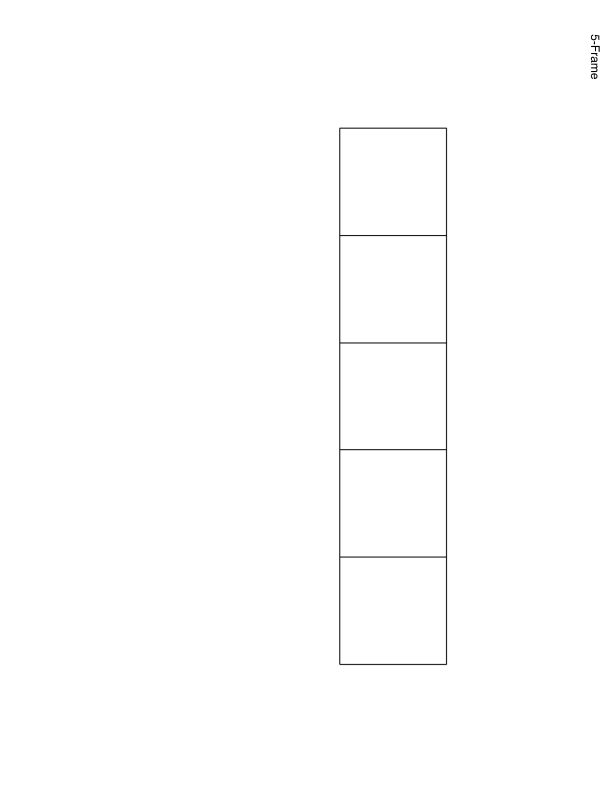
\includegraphics[trim=250 50 100 0, clip, width=0.45\linewidth]{external/blm/pdf-source/tablero-de-5.pdf}
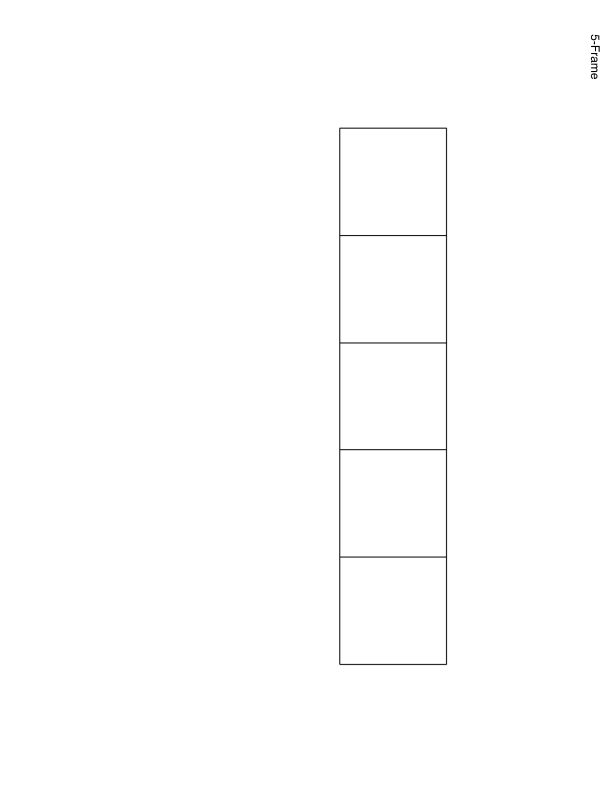
\includegraphics[trim=250 50 100 0, clip, width=0.45\linewidth]{external/blm/pdf-source/tablero-de-5.pdf}
\end{cutoutpage}
\end{activity}%
\end{subsubsectionptx}
\end{subsectionptx}
%
%
\typeout{************************************************}
\typeout{Subsección  Lección 4 -~Exploremos los bloques sólidos geométricos}
\typeout{************************************************}
%
\begin{subsectionptx}{Subsección}{Lección 4 -~Exploremos los bloques sólidos geométricos}{}{Lección 4}{}{}{lec-exploremosBloquesSolidosGeom}
%
%
\typeout{************************************************}
\typeout{Subsubsección  Actividad 2}
\typeout{************************************************}
%
\begin{subsubsectionptx}{Subsubsección}{Actividad 2}{}{Actividad 2}{}{}{lec-exploremosBloquesSolidosGeom-act2}
\begin{activity}{Actividad}{Conozcamos “Bloques sólidos geométricos: Construye lo que ves”.}{act-conozcamos-bloquesSolidosGeom-construyeVes}%
Usa bloques para construir una casa.%
\begin{image}{0}{1}{0}{}%
\includegraphics[max width=\linewidth, center]{external/png-source/house.png}
\end{image}%
% Más imágenes al final del libro.%
\begin{cutoutpage}[Tarjetas “Bloques sólidos geométricos: Construye lo que ves”]

\includegraphics[page=1, trim=60 250 35 80,clip, width=0.7\linewidth, center]{external/blm/pdf-source/bloques-solidos-geometricos-tarjetas.pdf}
\vfill
\noindent\rule{\linewidth}{0.4pt}
\vfill
\includegraphics[page=2, trim=60 250 35 60,clip, width=0.7\linewidth, center]{external/blm/pdf-source/bloques-solidos-geometricos-tarjetas.pdf}
\noindent\rule{\linewidth}{0.4pt}
\cleardoublepage

\includegraphics[page=3, trim=60 250 35 80,clip, width=0.7\linewidth, center]{external/blm/pdf-source/bloques-solidos-geometricos-tarjetas.pdf}
\vfill
\noindent\rule{\linewidth}{0.4pt}
\vfill
\includegraphics[page=4, trim=60 250 35 60,clip, width=0.7\linewidth, center]{external/blm/pdf-source/bloques-solidos-geometricos-tarjetas.pdf}
\noindent\rule{\linewidth}{0.4pt}
\cleardoublepage

\includegraphics[page=5, trim=60 250 35 80,clip, width=0.7\linewidth, center]{external/blm/pdf-source/bloques-solidos-geometricos-tarjetas.pdf}
\vfill
\noindent\rule{\linewidth}{0.4pt}
\vfill
\includegraphics[page=6, trim=60 250 35 60,clip, width=0.7\linewidth, center]{external/blm/pdf-source/bloques-solidos-geometricos-tarjetas.pdf}
\noindent\rule{\linewidth}{0.4pt}
\cleardoublepage

\includegraphics[page=7, trim=60 250 35 80,clip, width=0.7\linewidth, center]{external/blm/pdf-source/bloques-solidos-geometricos-tarjetas.pdf}
\vfill
\noindent\rule{\linewidth}{0.4pt}
\vfill
\includegraphics[page=8, trim=60 250 35 60,clip, width=0.7\linewidth, center]{external/blm/pdf-source/bloques-solidos-geometricos-tarjetas.pdf}
\noindent\rule{\linewidth}{0.4pt}
\cleardoublepage

\includegraphics[page=9, trim=60 250 35 90,clip, width=0.7\linewidth, center]{external/blm/pdf-source/bloques-solidos-geometricos-tarjetas.pdf}
\vfill
\noindent\rule{\linewidth}{0.4pt}
\vfill
\includegraphics[page=10, trim=60 250 35 60,clip, width=0.7\linewidth, center]{external/blm/pdf-source/bloques-solidos-geometricos-tarjetas.pdf}
\noindent\rule{\linewidth}{0.4pt}
\end{cutoutpage}
\end{activity}%
\end{subsubsectionptx}
\end{subsectionptx}
%
%
\typeout{************************************************}
\typeout{Subsección  Lección 5 -~Exploremos nuestras herramientas matemáticas}
\typeout{************************************************}
%
\begin{subsectionptx}{Subsección}{Lección 5 -~Exploremos nuestras herramientas matemáticas}{}{Lección 5}{}{}{lec-exploremosHerramientasMate}
%
%
\typeout{************************************************}
\typeout{Subsubsección  Actividad 1}
\typeout{************************************************}
%
\begin{subsubsectionptx}{Subsubsección}{Actividad 1}{}{Actividad 1}{}{}{lec-exploremosHerramientasMate-act1}
\begin{activity}{Actividad}{Conozcamos “Cubos encajables: Construye lo que ves”.}{act-conozcamos-construyeLoQueVes}%
\begin{image}{0}{1}{0}{-1\baselineskip}%
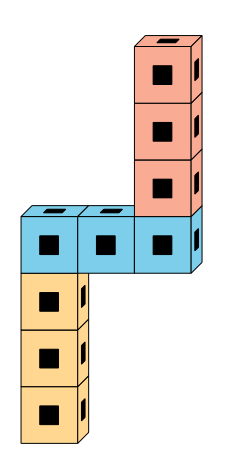
\includegraphics[max width=0.2\linewidth, center]{external/svg-source/tikz-file-148146.pdf}
\end{image}%
\begin{cutoutpage}[tarjetas para “Cubos encajables: Construye lo que ves”]
% \includegraphics[page=1, trim=60 250 35 80,clip, width=0.7\linewidth, center]{external/blm/pdf-source/bloques-solidos-geometricos-tarjetas.pdf}
\includegraphics[page=1, rotate=90, width=1.1\linewidth, center]{external/blm/tikz-source/cubos-encajables-tarjetas.pdf}
\cleardoublepage
\includegraphics[page=2, rotate=90, width=1.1\linewidth, center]{external/blm/tikz-source/cubos-encajables-tarjetas.pdf}
\cleardoublepage
\includegraphics[page=3, rotate=90, width=1.1\linewidth, center]{external/blm/tikz-source/cubos-encajables-tarjetas.pdf}
\end{cutoutpage}
\end{activity}%
\end{subsubsectionptx}
%
%
\typeout{************************************************}
\typeout{Subsubsección  Actividad 2}
\typeout{************************************************}
%
\begin{subsubsectionptx}{Subsubsección}{Actividad 2}{}{Actividad 2}{}{}{lec-exploremosHerramientasMate-act2}
\begin{activity}{Actividad}{Conozcamos “Fichas geométricas: Rompecabezas”.}{act-conozcamos-fichasGeometricas-rompecabezas}%
\begin{image}{0}{1}{0}{-1\baselineskip}%
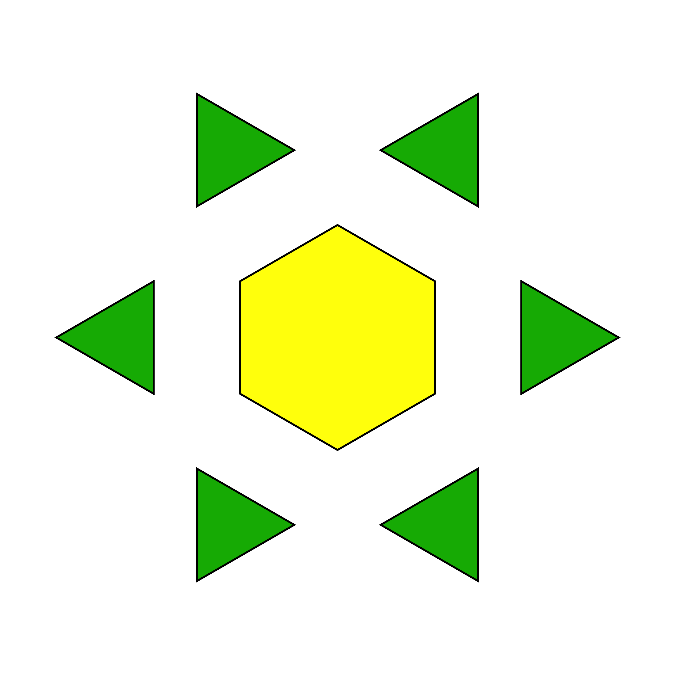
\includegraphics[max width=0.3\linewidth, center]{external/svg-source/tikz-file-148147.pdf}
\end{image}%
\end{activity}%
\begin{cutoutpage}[Tarjetas para “Fichas geométricas: Rompecabezas” (laminar por ambos lados)]
% \includegraphics[page=1, trim=60 250 35 80,clip, width=0.7\linewidth, center]{external/blm/pdf-source/bloques-solidos-geometricos-tarjetas.pdf}
\includegraphics[page=1, trim=0 0 0 40, clip, width=\linewidth, center]{external/blm/pdf-source/fichasGeometricas-rompecabezas.pdf}
\clearpage
\includegraphics[page=2, trim=0 0 0 40, clip, width=\linewidth, center]{external/blm/pdf-source/fichasGeometricas-rompecabezas.pdf}
\clearpage
\includegraphics[page=3, trim=0 0 0 40, clip, width=\linewidth, center]{external/blm/pdf-source/fichasGeometricas-rompecabezas.pdf}
\clearpage
\includegraphics[page=4, trim=0 0 0 40, clip, width=\linewidth, center]{external/blm/pdf-source/fichasGeometricas-rompecabezas.pdf}
\clearpage
\includegraphics[page=5, trim=0 0 0 40, clip, width=\linewidth, center]{external/blm/pdf-source/fichasGeometricas-rompecabezas.pdf}
\clearpage
\includegraphics[page=6, trim=0 0 0 40, clip, width=\linewidth, center]{external/blm/pdf-source/fichasGeometricas-rompecabezas.pdf}
\clearpage
\includegraphics[page=7, trim=0 0 0 40, clip, width=\linewidth, center]{external/blm/pdf-source/fichasGeometricas-rompecabezas.pdf}
\clearpage
\includegraphics[page=8, trim=0 0 0 40, clip, width=\linewidth, center]{external/blm/pdf-source/fichasGeometricas-rompecabezas.pdf}
\clearpage
\includegraphics[page=9, trim=0 0 0 40, clip, width=\linewidth, center]{external/blm/pdf-source/fichasGeometricas-rompecabezas.pdf}
\clearpage
\includegraphics[page=10, trim=0 0 0 40, clip, width=\linewidth, center]{external/blm/pdf-source/fichasGeometricas-rompecabezas.pdf}
\end{cutoutpage}
\end{subsubsectionptx}
\end{subsectionptx}
\end{sectionptx}
%
%
\typeout{************************************************}
\typeout{Sección  Sección B -~Reconozcamos cantidades}
\typeout{************************************************}
%
\begin{sectionptx}{Sección}{Sección B -~Reconozcamos cantidades}{}{Sección B -~Reconozcamos cantidades}{}{}{gra0-uni1-secB}
%
%
\typeout{************************************************}
\typeout{Subsección  Lección 6 -~Busquemos grupos pequeños}
\typeout{************************************************}
%
\begin{subsectionptx}{Subsección}{Lección 6 -~Busquemos grupos pequeños}{}{Lección 6}{}{}{lec-busquemosGruposMasPequenos}
\end{subsectionptx}
%
%
\typeout{************************************************}
\typeout{Subsección  Lección 7 -~Juego de búsqueda en el salón de clase}
\typeout{************************************************}
%
\begin{subsectionptx}{Subsección}{Lección 7 -~Juego de búsqueda en el salón de clase}{}{Lección 7}{}{}{lec-juegoBusqueda}
\end{subsectionptx}
%
%
\typeout{************************************************}
\typeout{Subsección  Lección 8 -~Grupos diferentes, misma cantidad}
\typeout{************************************************}
%
\begin{subsectionptx}{Subsección}{Lección 8 -~Grupos diferentes, misma cantidad}{}{Lección 8}{}{}{lec-gruposDiferentesMismaCantidad}
%
%
\typeout{************************************************}
\typeout{Subsubsección  Actividad 2}
\typeout{************************************************}
%
\begin{subsubsectionptx}{Subsubsección}{Actividad 2}{}{Actividad 2}{}{}{lec-gruposDiferentesMismaCantidad-act2}
\begin{activity}{Actividad}{Grupos diferentes, misma cantidad.}{act-gruposDiferentesMismaCantidad}%
\begin{image}{0}{1}{0}{}%
\includegraphics[max width=\linewidth, center]{external/png-source/K.1.C Beta Student Workbook.AnimalGroups.png}
\end{image}%
\begin{cutoutpage}[Tarjetas para "Grupos diferentes, misma cantidad" (recortar)]
\includegraphics[page=1, trim=55 35 35 0, clip, width=\linewidth, center]{external/blm/pdf-source/gruposDiferentesMismaCantidad.pdf}
\cleardoublepage
\includegraphics[page=2, trim=55 35 35 0, clip, width=\linewidth, center]{external/blm/pdf-source/gruposDiferentesMismaCantidad.pdf}
\cleardoublepage
\end{cutoutpage}
\end{activity}%
\end{subsubsectionptx}
\end{subsectionptx}
%
%
\typeout{************************************************}
\typeout{Subsección  Lección 9 -~Hagamos libros de imágenes}
\typeout{************************************************}
%
\begin{subsectionptx}{Subsección}{Lección 9 -~Hagamos libros de imágenes}{}{Lección 9}{}{}{lec-hagamosDeLibrosImagenes}
%
%
\typeout{************************************************}
\typeout{Subsubsección  Actividad 2}
\typeout{************************************************}
%
\begin{subsubsectionptx}{Subsubsección}{Actividad 2}{}{Actividad 2}{}{}{lec-hagamosDeLibrosImagenes-act2}
\begin{activity}{Actividad}{Conozcamos “Libros de imágenes: Crea”.}{act-conozcamos-librosDeImagenes-crea}%
Hojas del libro para crear en las páginas que siguen.
\end{activity}%
\clearpage
\includegraphics[page=2, rotate=90, trim=90 35 35 35, clip, width=\linewidth, center]{external/blm/pdf-source/center-picture-books-k-5-stage-2-create-picture-books-stage-2-recording-sheet.pdf}
\hrule
\includegraphics[page=1, rotate=90, trim=90 35 35 35, clip, width=\linewidth, center]{external/blm/pdf-source/center-picture-books-k-5-stage-2-create-picture-books-stage-2-recording-sheet.pdf}
\clearpage
\includegraphics[page=4, rotate=90, trim=90 35 35 35, clip, width=\linewidth, center]{external/blm/pdf-source/center-picture-books-k-5-stage-2-create-picture-books-stage-2-recording-sheet.pdf}
\hrule
\includegraphics[page=3, rotate=90, trim=90 35 35 35, clip, width=\linewidth, center]{external/blm/pdf-source/center-picture-books-k-5-stage-2-create-picture-books-stage-2-recording-sheet.pdf}
\end{subsubsectionptx}
\end{subsectionptx}
\end{sectionptx}
%
%
\typeout{************************************************}
\typeout{Sección  Sección C -~¿Hay suficientes?}
\typeout{************************************************}
%
\begin{sectionptx}{Sección}{Sección C -~¿Hay suficientes?}{}{Sección C -~¿Hay suficientes?}{}{}{gra0-uni1-secC}
%
%
\typeout{************************************************}
\typeout{Subsección  Lección 10 -~Cuántos ves: Construyamos sobre lo aprendido}
\typeout{************************************************}
%
\begin{subsectionptx}{Subsección}{Lección 10 -~Cuántos ves: Construyamos sobre lo aprendido}{}{Lección 10}{}{}{lec-cuantosVesConstruyamosSobreLoAprendido}
\end{subsectionptx}
%
%
\typeout{************************************************}
\typeout{Subsección  Lección 11 -~Consigamos suficientes}
\typeout{************************************************}
%
\begin{subsectionptx}{Subsección}{Lección 11 -~Consigamos suficientes}{}{Lección 11}{}{}{lec-consigamosSuficientes}
\end{subsectionptx}
\end{sectionptx}
%
%
\typeout{************************************************}
\typeout{Sección  Sección D -~Contemos colecciones}
\typeout{************************************************}
%
\begin{sectionptx}{Sección}{Sección D -~Contemos colecciones}{}{Sección D -~Contemos colecciones}{}{}{gra0-uni1-secD}
%
%
\typeout{************************************************}
\typeout{Subsección  Lección 12 -~¿Cuántos hay? (Parte 1)}
\typeout{************************************************}
%
\begin{subsectionptx}{Subsección}{Lección 12 -~¿Cuántos hay? (Parte 1)}{}{Lección 12}{}{}{lec-cuantosHayParte1}
%
%
\typeout{************************************************}
\typeout{Subsubsección  Actividad 1}
\typeout{************************************************}
%
\begin{subsubsectionptx}{Subsubsección}{Actividad 1}{}{Actividad 1}{}{}{lec-cuantosHayParte1-act1}
\begin{activity}{Actividad}{Contemos colecciones.}{act-contemosColecciones}%
¿Cuántos objetos hay en la colección?%
\par
\begin{cutoutpage}[tablero de conteo (laminar)]

\includegraphics[trim=100 70 50 60, clip, width=\linewidth, center]{external/blm/pdf-source/contemosColecciones-tableroDeConteo-countingMat.pdf}

\end{cutoutpage}
\end{activity}%
\end{subsubsectionptx}
%
%
% \typeout{************************************************}
% \typeout{Subsubsección  Actividad 2}
% \typeout{************************************************}
% %
% \begin{subsubsectionptx}{Subsubsección}{Actividad 2}{}{Actividad 2}{}{}{lec-cuantosHayParte1-act2}
% \begin{activity}{Actividad}{Contemos hasta 10 [Opcional].}{act-contemosHasta10}%
% Contemos juntos hasta 10%
% \end{activity}%
% \end{subsubsectionptx}
\typeout{************************************************}
\typeout{Subsubsección  Actividad 3}
\typeout{************************************************}
%
\begin{subsubsectionptx}{Subsubsección}{Actividad 3}{}{Actividad 3}{}{}{lec-cuantosHayParte1-act3}
\begin{activity}{Actividad}{Conozcamos “Fichas geométricas: Consigue y construye”.}{act-conozcamos-fichasGeometricas-consigueYConstruye}%
\begin{image}{0}{1}{0}{}%

\includegraphics[width=\linewidth]{external/svg-source/tikz-file-148183.pdf}
\end{image}%
\begin{image}{0}{1}{0}{}%

\includegraphics[width=\linewidth]{external/svg-source/tikz-file-148184.pdf}
\end{image}%
\begin{cutoutpage}[Tarjetas para Fichas geométricas: “Fichas geométricas: Consigue y construye” (laminar)]
\includegraphics[page=1, trim=10 30 50 50, clip, center]{external/blm/pdf-source/centro-fichasGeometricas-etapa3.pdf}
\clearpage
\includegraphics[page=2, trim=10 30 50 50, clip, center]{external/blm/pdf-source/centro-fichasGeometricas-etapa3.pdf}
\clearpage
\includegraphics[page=3, trim=10 30 50 50, clip, center]{external/blm/pdf-source/centro-fichasGeometricas-etapa3.pdf}
\clearpage
\includegraphics[page=4, trim=10 30 50 50, clip, center]{external/blm/pdf-source/centro-fichasGeometricas-etapa3.pdf}
\clearpage
\includegraphics[page=5, trim=10 30 50 50, clip, center]{external/blm/pdf-source/centro-fichasGeometricas-etapa3.pdf}
\clearpage
\includegraphics[page=6, trim=10 30 50 50, clip, center]{external/blm/pdf-source/centro-fichasGeometricas-etapa3.pdf}
\clearpage
\includegraphics[page=7, trim=10 30 50 50, clip, center]{external/blm/pdf-source/centro-fichasGeometricas-etapa3.pdf}
\clearpage
\includegraphics[page=8, trim=10 30 50 50, clip, center]{external/blm/pdf-source/centro-fichasGeometricas-etapa3.pdf}
\clearpage
\includegraphics[page=9, trim=10 30 50 50, clip, center]{external/blm/pdf-source/centro-fichasGeometricas-etapa3.pdf}
\clearpage
\includegraphics[page=10, trim=10 30 50 50, clip, center]{external/blm/pdf-source/centro-fichasGeometricas-etapa3.pdf}
\clearpage
\end{cutoutpage}
\end{activity}%
\end{subsubsectionptx}
\end{subsectionptx}
%
%
\typeout{************************************************}
\typeout{Subsección  Lección 13 -~¿Cuántos hay? (Parte 2)}
\typeout{************************************************}
%
\begin{subsectionptx}{Subsección}{Lección 13 -~¿Cuántos hay? (Parte 2)}{}{Lección 13}{}{}{lec-cuantosHayParte2}
%
%
\typeout{************************************************}
\typeout{Subsubsección  Actividad 1}
\typeout{************************************************}
%
\begin{subsubsectionptx}{Subsubsección}{Actividad 1}{}{Actividad 1}{}{}{lec-cuantosHayParte2-act1}
\begin{activity}{Actividad}{Contemos colecciones.}{act-contemosColecciones2}%
Contemos otra colección de objetos%
\end{activity}%
\end{subsubsectionptx}
\end{subsectionptx}
%
%
\typeout{************************************************}
\typeout{Subsección  Lección 14 -~Respondamos preguntas tipo “¿Cuántos?”}
\typeout{************************************************}
%
\begin{subsectionptx}{Subsección}{Lección 14 -~Respondamos preguntas tipo “¿Cuántos?”}{}{Lección 14}{}{}{lec-preguntasTipoCuantos}
%
%
\typeout{************************************************}
\typeout{Subsubsección  Actividad 1}
\typeout{************************************************}
%
\begin{subsubsectionptx}{Subsubsección}{Actividad 1}{}{Actividad 1}{}{}{lec-preguntasTipoCuantos-act1}
\begin{activity}{Actividad}{Contemos colecciones: ¿Cuántos?}{act-contemosColecciones-cuantos}%
¿Cuántos objetos hay en tu colección?%
\end{activity}%
\end{subsubsectionptx}
%
%
\typeout{************************************************}
\typeout{Subsubsección  Actividad 2}
\typeout{************************************************}
%
\begin{subsubsectionptx}{Subsubsección}{Actividad 2}{}{Actividad 2}{}{}{lec-preguntasTipoCuantos-act2}
\begin{activity}{Actividad}{Contemos cajas de huevos.}{act-contarCajasHuevos}%
Usen la caja de huevos para descubrir cuántos objetos hay en su colección%
\begin{cutoutpage}[alternativa de caja de huevos para contar]
\includegraphics[trim=180 30 50 50, clip, center]{external/blm/pdf-source/contemos-cajasDeHuevos.pdf}
\end{cutoutpage}
\end{activity}%
\end{subsubsectionptx}
%
%
\typeout{************************************************}
\typeout{Subsubsección  Actividad 3}
\typeout{************************************************}
%
\begin{subsubsectionptx}{Subsubsección}{Actividad 3}{}{Actividad 3}{}{}{lec-preguntasTipoCuantos-act3}
\begin{activity}{Actividad}{Conozcamos “Cubos encajables: Consigue y construye”.}{act-conozcamos-cubosEncajables-consigueConstruye}%
\begin{image}{0}{1}{0}{}%
\includegraphics[max width=\linewidth, center]{external/svg-source/tikz-file-148187.pdf}
\end{image}%
\begin{image}{0}{1}{0}{}%
\includegraphics[max width=\linewidth, center]{external/svg-source/tikz-file-148188.pdf}
\end{image}%
\begin{cutoutpage}[hojas para “Cubos encajables: Consigue y construye” (laminar)]
\includegraphics[page=1, trim=30 60 30 35, clip, center]{external/blm/pdf-source/centro-cubosEncajables-consigueYConstruye.pdf}
\clearpage
\includegraphics[page=2, trim=30 60 30 35, clip, center]{external/blm/pdf-source/centro-cubosEncajables-consigueYConstruye.pdf}
\clearpage
\includegraphics[page=3, trim=30 60 30 35, clip, center]{external/blm/pdf-source/centro-cubosEncajables-consigueYConstruye.pdf}
\clearpage
\includegraphics[page=4, trim=30 60 30 35, clip, center]{external/blm/pdf-source/centro-cubosEncajables-consigueYConstruye.pdf}
\clearpage
\includegraphics[page=5, trim=30 60 30 35, clip, center]{external/blm/pdf-source/centro-cubosEncajables-consigueYConstruye.pdf}
\clearpage
\includegraphics[page=6, trim=30 60 30 35, clip, center]{external/blm/pdf-source/centro-cubosEncajables-consigueYConstruye.pdf}
\clearpage
\includegraphics[page=7, trim=30 60 30 35, clip, center]{external/blm/pdf-source/centro-cubosEncajables-consigueYConstruye.pdf}
\clearpage
\includegraphics[page=8, trim=30 60 30 35, clip, center]{external/blm/pdf-source/centro-cubosEncajables-consigueYConstruye.pdf}
\clearpage
\includegraphics[page=9, trim=30 60 30 35, clip, center]{external/blm/pdf-source/centro-cubosEncajables-consigueYConstruye.pdf}
\clearpage
\includegraphics[page=10, trim=30 60 30 35, clip, center]{external/blm/pdf-source/centro-cubosEncajables-consigueYConstruye.pdf}
\end{cutoutpage}
\end{activity}%
\end{subsubsectionptx}
\end{subsectionptx}
%
%
\typeout{************************************************}
\typeout{Subsección  Lección 15 -~Expliquemos cómo contamos}
\typeout{************************************************}
%
\begin{subsectionptx}{Subsección}{Lección 15 -~Expliquemos cómo contamos}{}{Lección 15}{}{}{lec-explicarConteo}
%
%
\typeout{************************************************}
\typeout{Subsubsección  Actividad 1}
\typeout{************************************************}
%
\begin{subsubsectionptx}{Subsubsección}{Actividad 1}{}{Actividad 1}{}{}{lec-explicarConteo-act1}
\begin{activity}{Actividad}{Contemos colecciones: Comparte cómo contaste.}{act-contemosColecciones-comparteConteo}%
¿Cuántos objetos hay en su colección?%
\end{activity}%
\end{subsubsectionptx}
%
%
\typeout{************************************************}
\typeout{Subsubsección  Actividad 2}
\typeout{************************************************}
%
\begin{subsubsectionptx}{Subsubsección}{Actividad 2}{}{Actividad 2}{}{}{lec-explicarConteo-act2}
\begin{activity}{Actividad}{Usemos un tablero de conteo para llevar la cuenta [Opcional].}{act-tableroConteoLlevarCuenta}%
Usemos un tablero de conteo.%
\end{activity}%
\end{subsubsectionptx}
\end{subsectionptx}
%
%
\typeout{************************************************}
\typeout{Subsección  Lección 16 -~Representemos nuestras colecciones}
\typeout{************************************************}
%
\begin{subsectionptx}{Subsección}{Lección 16 -~Representemos nuestras colecciones}{}{Lección 16}{}{}{lec-representarColecciones}
%
%
\typeout{************************************************}
\typeout{Subsubsección  Actividad 1}
\typeout{************************************************}
%
\begin{subsubsectionptx}{Subsubsección}{Actividad 1}{}{Actividad 1}{}{}{lec-representarColecciones-act1}
\begin{activity}{Actividad}{Contemos colecciones: Muestra cuántos.}{act-contemosColecciones-muestraCuantos}%
¿Cuántos objetos hay en su colección?%
\end{activity}%
\end{subsubsectionptx}
%
%
\typeout{************************************************}
\typeout{Subsubsección  Actividad 2}
\typeout{************************************************}
%
\begin{subsubsectionptx}{Subsubsección}{Actividad 2}{}{Actividad 2}{}{}{lec-representarColecciones-act2}
\begin{activity}{Actividad}{Respondamos preguntas tipo "¿Cuántos?".}{act-preguntasTipoCuantos}%
¿Cuántos objetos hay en su colección?%
\end{activity}%
\end{subsubsectionptx}
\end{subsectionptx}
%
%
\typeout{************************************************}
\typeout{Subsección  Lección 17 -~Esculturas con cubos encajables (opcional)}
\typeout{************************************************}
%
\begin{subsectionptx}{Subsección}{Lección 17 -~Esculturas con cubos encajables (opcional)}{}{Lección 17}{}{}{lec-esculturasCubosEncajables}
%
%
\typeout{************************************************}
\typeout{Subsubsección  Actividad 1}
\typeout{************************************************}
%
\begin{subsubsectionptx}{Subsubsección}{Actividad 1}{}{Actividad 1}{}{}{lec-esculturasCubosEncajables-act1}
\begin{activity}{Actividad}{Contemos cubos.}{act-conectemosCubosEncajables}%
¿Cuántos cubos hay en tu colección?%
\end{activity}%
\end{subsubsectionptx}
%
%
\typeout{************************************************}
\typeout{Subsubsección  Actividad 2}
\typeout{************************************************}
%
\begin{subsubsectionptx}{Subsubsección}{Actividad 2}{}{Actividad 2}{}{}{lec-esculturasCubosEncajables-act2}
\begin{activity}{Actividad}{Creaciones con cubos encajables.}{act-creacionesCubosEncajables}%
Usa todos tus cubos encajables para crear lo que quieras.%
\end{activity}%
\end{subsubsectionptx}
\end{subsectionptx}
\end{sectionptx}
%
%

%
\typeout{************************************************}
\typeout{Referencias  Atribuciones de imágenes}
\typeout{************************************************}
%
\clearpage
\begin{references-section}{Referencias}{Atribuciones de imágenes}{}{Atribuciones de imágenes}{}{}{gra0-uni1-9}
Las imágenes sin atrubición las produjo LEMA \href{https://www.grupolema.org}{www.grupolema.org}\footnote{\nolinkurl{www.grupolema.org}\label{gra0-uni1-9-2-2}} específicamente para esta adaptación y se liberan con una licencia Creative Commons Attribution 4.0 International License (CC BY 4.0), o son © 2021 \href{https://curriculum.illustrativemathematics.org}{Illustrative Mathematics}\footnote{\nolinkurl{curriculum.illustrativemathematics.org}\label{gra0-uni1-9-2-4}} con una licencia Creative Commons Attribution 4.0 International License (CC BY 4.0) y se reproducen directamente de la versión en Español disponible en \href{https://im.kendallhunt.com/K5_ES/curriculum.html}{im.kendallhunt.com}\footnote{\nolinkurl{im.kendallhunt.com/K5_ES/curriculum.html}\label{gra0-uni1-9-2-6}}.%
\end{references-section}
%
%

\end{document}
